\section{Silicon Strip Detector (SSD)}

O Silicon Strip Detector πρόκειται για ένα τέταρτο στρώμα ανιχνευτών που συμπληρώνουν τα τρια του SVT φτιάχνοντας έτσι ένα σύστημα ιχνηλάτησης των τροχιών εντός του TPC.
	Παρέχει διδιάστατη απεικόνιση των δευτερευοντων σωματιδίων, προεκτείνοντας τις ανακατασκευαστική τροχιών από τον SVT, ενώ ταυτόχρονα κάνει και μετρήσεις απώλειας ενέργειας. Επίσης, βελτιώνει την αποδοτικότητα ανίχνευσης τροχιών στην κεντρικη περιοχή και για σωματίδια χαμληής ορμής.
	Είναι τοποθετημένος μόλις 230mm από την δέσμη και καλύπτει μία περιοχή pseudorapidity $|\eta|<1.2$ για την οποία χρειάζεται συνολική επιφάνεια Si 1$m^2$.
		
	
		\begin{figure}[h!]
    \centering
    \begin{minipage}{.5\textwidth}
        \centering
        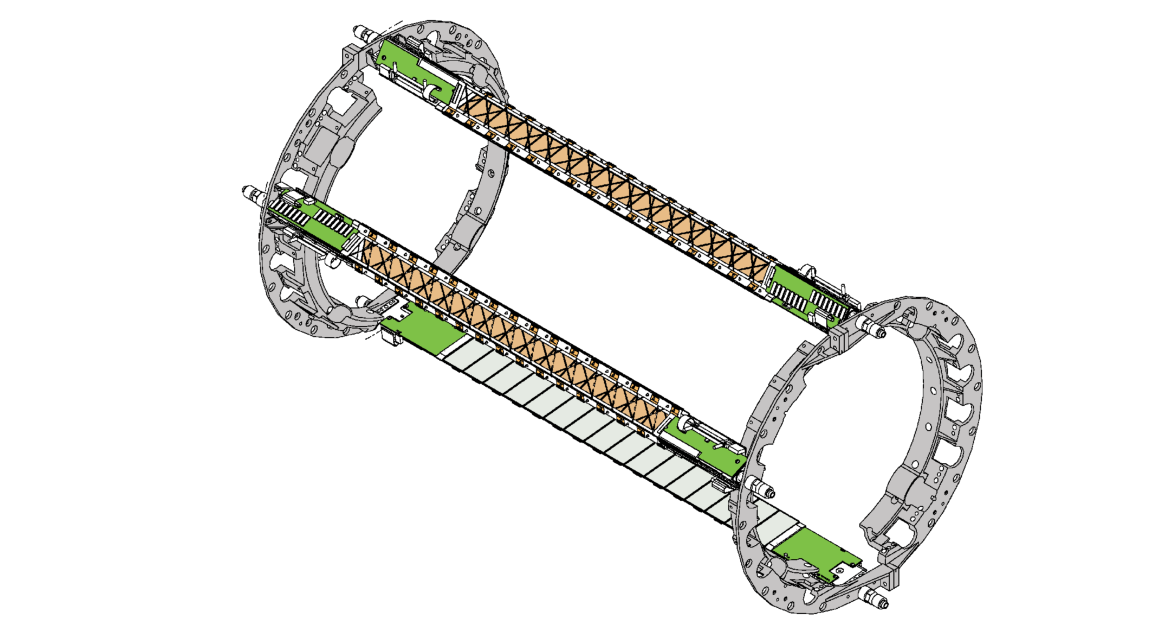
\includegraphics[width=0.9\linewidth, height=0.25\textheight]{STAR_Detectors/SSD_full}
        \caption{Ο SSD με 3 από τις 20 ράβδους}
        \label{fig3.16}
    \end{minipage}%
    \begin{minipage}{0.5\textwidth}
        \centering
        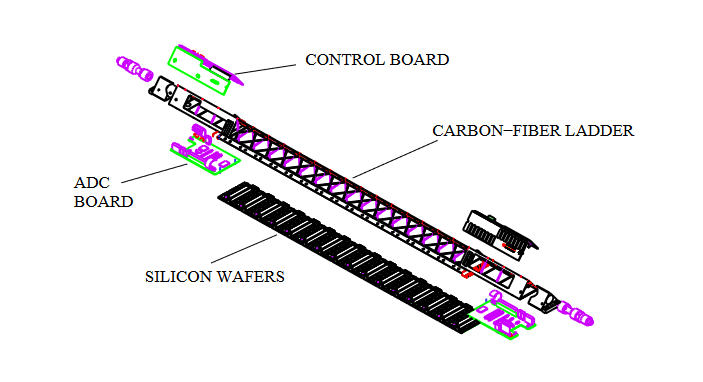
\includegraphics[width=0.9\linewidth, height=0.25\textheight]{STAR_Detectors/SSD_ladder}
        \caption{Η δομή μίας ράβδου του SSD}
        \label{fig3.17}
    \end{minipage}
\end{figure}

	Αποτελείται από 2 ημικυλινδρικά μέρη το κάθενα εκ των οποίων έχει 10 ράβδους. Η κάθε ράβδος στηρίζει 16 τμήματα ανιχνευτών μονάδων απο Πυρίτιο με πάχος 300μm. Η κάθε μονάδα αποτελείται από Πυρίτιο στον κύριο όγκο της, το οποίο είναι και το μέσο στο οποίο γίνονται οι αλληλεπιδράσεις των πρωτεύοντων σωματιδίων και παράγονται τα δευτερεύοντα τα οποία και ανιχνεύουμε. Στις άκρες του κύριου όγκου υπάρχουν λωρίδες διόδων στις οποίες συγκεντώνονται οι φορείς λόγω διάχυσης η οποία προσανατολίζεται από το ηλεκτρικό πεδίο που υπάρχει λόγω των διόδων. Αν τοποθετήσουμε λωρίδες και από τις δύο πλευρές, τότε  καταγράφουμε διπλάσια πληροφορία για το εσωτερικό του ανιχνευτή, συνεπώς έχουμε καλύτερη διακριτική ικανότητα. 
	
	
	
	\begin{figure}[h!]
	    \centering
	    \begin{minipage}{.5\textwidth}
	        \centering
	        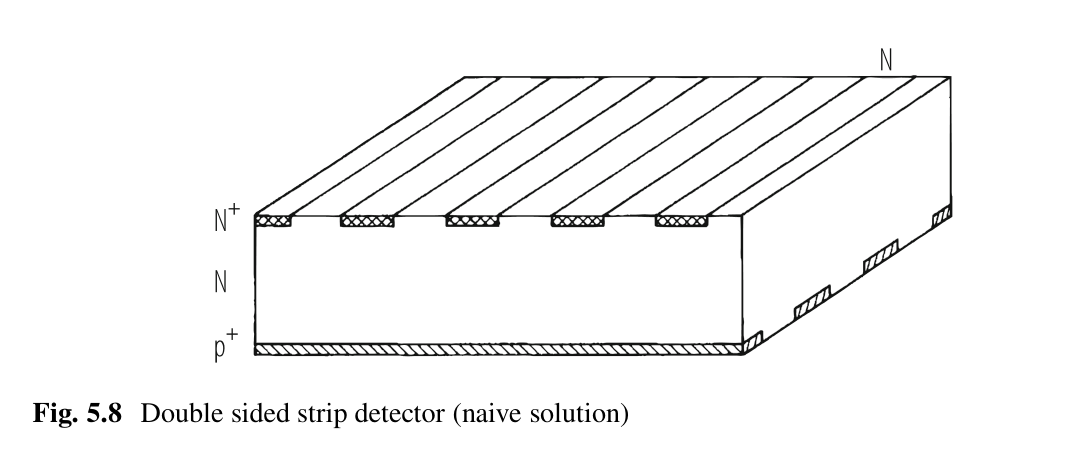
\includegraphics[width=0.9\linewidth, height=0.25\textheight]{STAR_Detectors/SSD_naive}
	        \caption{Μία απλή εκδοχή μίας μονάδας SSD}
	        \label{fig3.19}
	    \end{minipage}%
	    \begin{minipage}{0.5\textwidth}
	        \centering
	        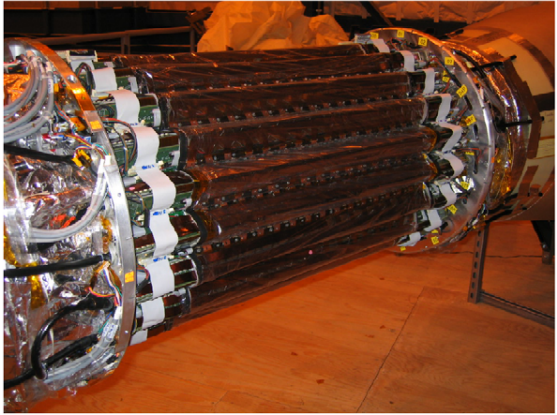
\includegraphics[width=0.9\linewidth, height=0.25\textheight]{STAR_Detectors/SSD_image}
	        \caption{Εικόνα του SSD πριν την εγκατάσταση στο STAR}
	        \label{fig3.20}
	    \end{minipage}
	\end{figure}
	
 	Ένα από τα προβλήματα που προκύπτουν σε έναν τέτοιο ανιχνευτή είναι ότι συσσωρεύονται πολλά ηλεκτρόνια τριγύρω από τις λωρίδες ημιαγωγού τύπου n. για να λύσουμε αυτό το πρόβλημα μπορούμε να εμφυτέψουμε ημιαγωγό τύπου p ενδιάμεσα από τις λωρίδες τύπου n και τότε απομακρύνονται ευκολότερα από την ενδιάμεση περιοχή προς τις διόδους.
 	 
	